\documentclass[twoside]{book}

% Packages required by doxygen
\usepackage{calc}
\usepackage{doxygen}
\usepackage{graphicx}
\usepackage[utf8]{inputenc}
\usepackage{makeidx}
\usepackage{multicol}
\usepackage{multirow}
\usepackage{textcomp}
\usepackage[table]{xcolor}

% Font selection
\usepackage[T1]{fontenc}
\usepackage{mathptmx}
\usepackage[scaled=.90]{helvet}
\usepackage{courier}
\usepackage{amssymb}
\usepackage{sectsty}
\renewcommand{\familydefault}{\sfdefault}
\allsectionsfont{%
  \fontseries{bc}\selectfont%
  \color{darkgray}%
}
\renewcommand{\DoxyLabelFont}{%
  \fontseries{bc}\selectfont%
  \color{darkgray}%
}

% Page & text layout
\usepackage{geometry}
\geometry{%
  a4paper,%
  top=2.5cm,%
  bottom=2.5cm,%
  left=2.5cm,%
  right=2.5cm%
}
\tolerance=750
\hfuzz=15pt
\hbadness=750
\setlength{\emergencystretch}{15pt}
\setlength{\parindent}{0cm}
\setlength{\parskip}{0.2cm}
\makeatletter
\renewcommand{\paragraph}{%
  \@startsection{paragraph}{4}{0ex}{-1.0ex}{1.0ex}{%
    \normalfont\normalsize\bfseries\SS@parafont%
  }%
}
\renewcommand{\subparagraph}{%
  \@startsection{subparagraph}{5}{0ex}{-1.0ex}{1.0ex}{%
    \normalfont\normalsize\bfseries\SS@subparafont%
  }%
}
\makeatother

% Headers & footers
\usepackage{fancyhdr}
\pagestyle{fancyplain}
\fancyhead[LE]{\fancyplain{}{\bfseries\thepage}}
\fancyhead[CE]{\fancyplain{}{}}
\fancyhead[RE]{\fancyplain{}{\bfseries\leftmark}}
\fancyhead[LO]{\fancyplain{}{\bfseries\rightmark}}
\fancyhead[CO]{\fancyplain{}{}}
\fancyhead[RO]{\fancyplain{}{\bfseries\thepage}}
\fancyfoot[LE]{\fancyplain{}{}}
\fancyfoot[CE]{\fancyplain{}{}}
\fancyfoot[RE]{\fancyplain{}{\bfseries\scriptsize Generated on Sat Aug 19 2017 23\-:34\-:13 for Machine Learning C++ by Doxygen }}
\fancyfoot[LO]{\fancyplain{}{\bfseries\scriptsize Generated on Sat Aug 19 2017 23\-:34\-:13 for Machine Learning C++ by Doxygen }}
\fancyfoot[CO]{\fancyplain{}{}}
\fancyfoot[RO]{\fancyplain{}{}}
\renewcommand{\footrulewidth}{0.4pt}
\renewcommand{\chaptermark}[1]{%
  \markboth{#1}{}%
}
\renewcommand{\sectionmark}[1]{%
  \markright{\thesection\ #1}%
}

% Indices & bibliography
\usepackage{natbib}
\usepackage[titles]{tocloft}
\setcounter{tocdepth}{3}
\setcounter{secnumdepth}{5}
\makeindex

% Hyperlinks (required, but should be loaded last)
\usepackage{ifpdf}
\ifpdf
  \usepackage[pdftex,pagebackref=true]{hyperref}
\else
  \usepackage[ps2pdf,pagebackref=true]{hyperref}
\fi
\hypersetup{%
  colorlinks=true,%
  linkcolor=blue,%
  citecolor=blue,%
  unicode%
}

% Custom commands
\newcommand{\clearemptydoublepage}{%
  \newpage{\pagestyle{empty}\cleardoublepage}%
}


%===== C O N T E N T S =====

\begin{document}

% Titlepage & ToC
\hypersetup{pageanchor=false}
\pagenumbering{roman}
\begin{titlepage}
\vspace*{7cm}
\begin{center}%
{\Large Machine Learning C++ }\\
\vspace*{1cm}
{\large Generated by Doxygen 1.8.6}\\
\vspace*{0.5cm}
{\small Sat Aug 19 2017 23:34:13}\\
\end{center}
\end{titlepage}
\clearemptydoublepage
\tableofcontents
\clearemptydoublepage
\pagenumbering{arabic}
\hypersetup{pageanchor=true}

%--- Begin generated contents ---
\chapter{M\-Lcpp}
\label{md__home_jiguangshen_HPC_MachineLearning_MLcpp_src_README}
\hypertarget{md__home_jiguangshen_HPC_MachineLearning_MLcpp_src_README}{}
A Machine Learning Library written in C++ Practice the state-\/of-\/art machine learning algorithms in C++ (Growing weekly by 1 or 2 algorithms).

Algorithms included\-:
\begin{DoxyItemize}
\item Artificial neural network
\item Support vector machines
\end{DoxyItemize}

\section*{Step one\-: Set up the third party libraries}


\begin{DoxyItemize}
\item Boost C++ libraries 
\end{DoxyItemize}
\chapter{Hierarchical Index}
\section{Class Hierarchy}
This inheritance list is sorted roughly, but not completely, alphabetically\-:\begin{DoxyCompactList}
\item \contentsline{section}{bpnet}{\pageref{classbpnet}}{}
\begin{DoxyCompactList}
\item \contentsline{section}{bpnet\-\_\-\-Cross\-Entropy\-\_\-softmax}{\pageref{classbpnet__CrossEntropy__softmax}}{}
\item \contentsline{section}{bpnet\-\_\-\-M\-S\-E\-\_\-sigmoid}{\pageref{classbpnet__MSE__sigmoid}}{}
\end{DoxyCompactList}
\item \contentsline{section}{dataframe}{\pageref{structdataframe}}{}
\begin{DoxyCompactList}
\item \contentsline{section}{banknote\-\_\-data}{\pageref{structbanknote__data}}{}
\item \contentsline{section}{iris\-\_\-data}{\pageref{structiris__data}}{}
\end{DoxyCompactList}
\item \contentsline{section}{layer}{\pageref{structlayer}}{}
\begin{DoxyCompactList}
\item \contentsline{section}{layer\-\_\-sigmoid}{\pageref{structlayer__sigmoid}}{}
\item \contentsline{section}{layer\-\_\-softmax}{\pageref{structlayer__softmax}}{}
\item \contentsline{section}{layer\-\_\-tanh}{\pageref{structlayer__tanh}}{}
\end{DoxyCompactList}
\item \contentsline{section}{neuron}{\pageref{structneuron}}{}
\end{DoxyCompactList}

\chapter{Class Index}
\section{Class List}
Here are the classes, structs, unions and interfaces with brief descriptions\-:\begin{DoxyCompactList}
\item\contentsline{section}{\hyperlink{structabalone__data}{abalone\-\_\-data} \\*The U\-C\-I data abalone data set }{\pageref{structabalone__data}}{}
\item\contentsline{section}{\hyperlink{classbpnet}{bpnet} \\*A backpropagation neural network class The back-\/propagation network has the architecture of three components propagate, update and train }{\pageref{classbpnet}}{}
\item\contentsline{section}{\hyperlink{classbpnet__CrossEntropy__softmax}{bpnet\-\_\-\-Cross\-Entropy\-\_\-softmax} \\*Child class, backpropagation foward feed nerual net using croos entropy loss and softmax activation. Usually a good choice for multi-\/classification problems }{\pageref{classbpnet__CrossEntropy__softmax}}{}
\item\contentsline{section}{\hyperlink{classbpnet__MSE__sigmoid}{bpnet\-\_\-\-M\-S\-E\-\_\-sigmoid} \\*Child class, backpropagation foward feed nerual net using mean squared error loss and sigmoid activation. Usually a good choice for binary classification problems }{\pageref{classbpnet__MSE__sigmoid}}{}
\item\contentsline{section}{\hyperlink{structdataframe}{dataframe} \\*The data framework for classification problems. It defines the way to load data and handle categorical class variables and display data info }{\pageref{structdataframe}}{}
\item\contentsline{section}{\hyperlink{structlayer}{layer} }{\pageref{structlayer}}{}
\item\contentsline{section}{\hyperlink{structlayer__sigmoid}{layer\-\_\-sigmoid} }{\pageref{structlayer__sigmoid}}{}
\item\contentsline{section}{\hyperlink{structlayer__softmax}{layer\-\_\-softmax} }{\pageref{structlayer__softmax}}{}
\item\contentsline{section}{\hyperlink{structlayer__tanh}{layer\-\_\-tanh} }{\pageref{structlayer__tanh}}{}
\item\contentsline{section}{\hyperlink{structneuron}{neuron} }{\pageref{structneuron}}{}
\end{DoxyCompactList}

\chapter{Class Documentation}
\hypertarget{structabalone__data}{\section{abalone\-\_\-data Struct Reference}
\label{structabalone__data}\index{abalone\-\_\-data@{abalone\-\_\-data}}
}


The U\-C\-I data abalone data set.  




{\ttfamily \#include $<$abalone.\-h$>$}

Inheritance diagram for abalone\-\_\-data\-:\begin{figure}[H]
\begin{center}
\leavevmode
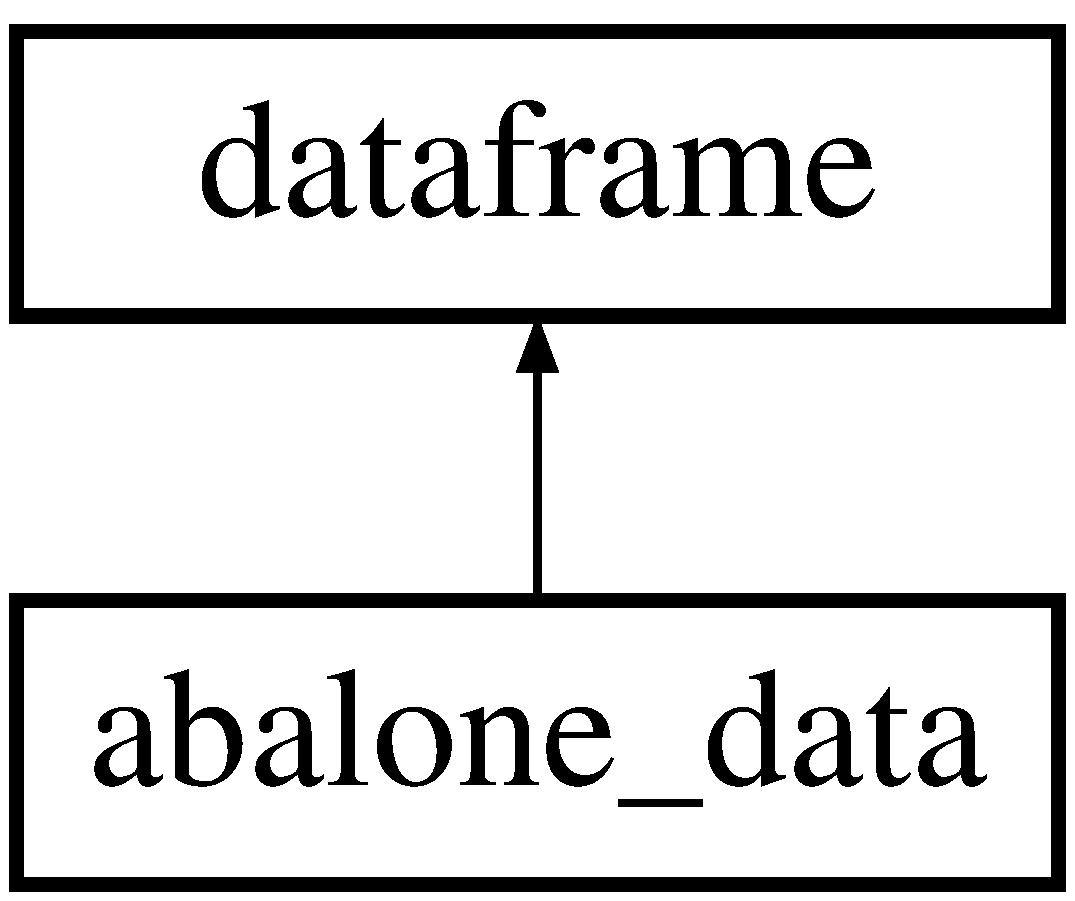
\includegraphics[height=2.000000cm]{structabalone__data}
\end{center}
\end{figure}
\subsection*{Public Member Functions}
\begin{DoxyCompactItemize}
\item 
void \hyperlink{structabalone__data_a2a4ddb71a6bd1126467bf3c9645f6591}{load} (std\-::string \&path)
\item 
void \hyperlink{structabalone__data_aff9641cf77f835161642a8a37e6ddc39}{data\-\_\-info} ()
\end{DoxyCompactItemize}
\subsection*{Additional Inherited Members}


\subsection{Detailed Description}
The U\-C\-I data abalone data set. 

\subsection{Member Function Documentation}
\hypertarget{structabalone__data_aff9641cf77f835161642a8a37e6ddc39}{\index{abalone\-\_\-data@{abalone\-\_\-data}!data\-\_\-info@{data\-\_\-info}}
\index{data\-\_\-info@{data\-\_\-info}!abalone_data@{abalone\-\_\-data}}
\subsubsection[{data\-\_\-info}]{\setlength{\rightskip}{0pt plus 5cm}void abalone\-\_\-data\-::data\-\_\-info (
\begin{DoxyParamCaption}
{}
\end{DoxyParamCaption}
)\hspace{0.3cm}{\ttfamily [virtual]}}}\label{structabalone__data_aff9641cf77f835161642a8a37e6ddc39}
print data info 

Reimplemented from \hyperlink{structdataframe_ac71cab6be91e8cb90d8efa88e6866b83}{dataframe}.

\hypertarget{structabalone__data_a2a4ddb71a6bd1126467bf3c9645f6591}{\index{abalone\-\_\-data@{abalone\-\_\-data}!load@{load}}
\index{load@{load}!abalone_data@{abalone\-\_\-data}}
\subsubsection[{load}]{\setlength{\rightskip}{0pt plus 5cm}void abalone\-\_\-data\-::load (
\begin{DoxyParamCaption}
\item[{std\-::string \&}]{path}
\end{DoxyParamCaption}
)\hspace{0.3cm}{\ttfamily [virtual]}}}\label{structabalone__data_a2a4ddb71a6bd1126467bf3c9645f6591}
load data from file 
\begin{DoxyParams}{Parameters}
{\em path} & string path to file \\
\hline
\end{DoxyParams}


Reimplemented from \hyperlink{structdataframe_ae108c949f6f3f89c7ed000e90c3a2e64}{dataframe}.



The documentation for this struct was generated from the following files\-:\begin{DoxyCompactItemize}
\item 
/home/jiguangshen/\-H\-P\-C\-\_\-\-Machine\-Learning/\-M\-Lcpp/src/examples/abalone.\-h\item 
/home/jiguangshen/\-H\-P\-C\-\_\-\-Machine\-Learning/\-M\-Lcpp/src/examples/abalone.\-cpp\end{DoxyCompactItemize}

\hypertarget{classbpnet}{\section{bpnet Class Reference}
\label{classbpnet}\index{bpnet@{bpnet}}
}


A backpropagation neural network class The back-\/propagation network has the architecture of three components propagate, update and train.  




{\ttfamily \#include $<$nnet.\-h$>$}

Inheritance diagram for bpnet\-:\begin{figure}[H]
\begin{center}
\leavevmode
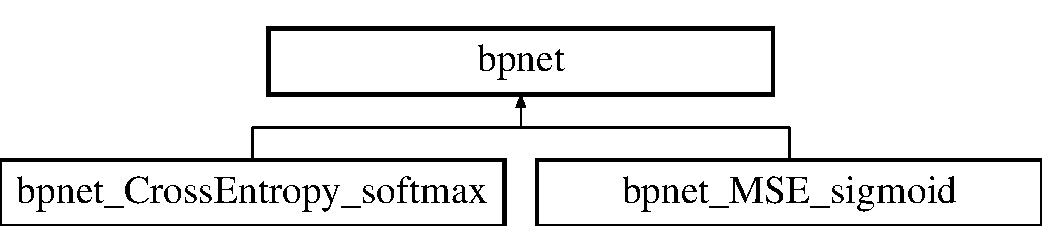
\includegraphics[height=2.000000cm]{classbpnet}
\end{center}
\end{figure}
\subsection*{Public Member Functions}
\begin{DoxyCompactItemize}
\item 
\hyperlink{classbpnet_adfeeece0abde65630da85276488cc0b2}{bpnet} (int \-\_\-n\-\_\-input, int \-\_\-n\-\_\-neurons\-\_\-in, int \-\_\-n\-\_\-output, std\-::vector$<$ int $>$ \-\_\-hidden\-\_\-layers, int \-\_\-n\-\_\-hidden\-\_\-layers)
\item 
virtual \hyperlink{classbpnet_a7189286dfd5cfdd648bcc8c78a177891}{$\sim$bpnet} ()
\item 
virtual void \hyperlink{classbpnet_a3731e200c3191fc77be85f1db2c2d4f9}{create} ()
\item 
virtual int \hyperlink{classbpnet_aa35c06d999256c9aebeed4f38bca9d0f}{get\-\_\-n\-\_\-hidden\-\_\-layers} ()
\item 
void \hyperlink{classbpnet_a77cd3c63e9948e4b6cc9e3a0412e25ea}{propagate} (const std\-::vector$<$ double $>$ \&input)
\item 
void \hyperlink{classbpnet_a87beae9040de4815cbcada7420f0df2a}{update} (int layer\-\_\-index)
\item 
virtual double \hyperlink{classbpnet_a653eae04b7dcfb4271421fd079849f89}{train} (const std\-::vector$<$ double $>$ \&train\-\_\-data, const std\-::vector$<$ double $>$ \&train\-\_\-class, double learning\-\_\-rate, double momentum)
\item 
virtual void \hyperlink{classbpnet_a9da604c278a2d583511071fdc754c9c6}{get\-\_\-output} (std\-::vector$<$ double $>$ \&input, std\-::vector$<$ double $>$ \&output)
\end{DoxyCompactItemize}
\subsection*{Protected Attributes}
\begin{DoxyCompactItemize}
\item 
std\-::unique\-\_\-ptr$<$ \hyperlink{structlayer}{layer} $>$ \hyperlink{classbpnet_aeb161ecafe664d9f6e0d188b94c778f4}{input\-\_\-layer}
\item 
std\-::unique\-\_\-ptr$<$ \hyperlink{structlayer}{layer} $>$ \hyperlink{classbpnet_afc882a791c00244a5b5f0ff8badcbc1e}{output\-\_\-layer}
\item 
std\-::vector$<$ std\-::unique\-\_\-ptr\\*
$<$ \hyperlink{structlayer}{layer} $>$ $>$ \hyperlink{classbpnet_a9f1d31d7cdb034587768016a799c36f6}{hidden\-\_\-layers}
\item 
\hypertarget{classbpnet_aa4e55fef61fe2886ea6d860a1e4d63f4}{int {\bfseries n\-\_\-hidden\-\_\-layers}}\label{classbpnet_aa4e55fef61fe2886ea6d860a1e4d63f4}

\item 
\hypertarget{classbpnet_afa95293a45b21300a96d762f69232e2d}{int {\bfseries n\-\_\-input}}\label{classbpnet_afa95293a45b21300a96d762f69232e2d}

\item 
\hypertarget{classbpnet_a30a2996bef81fa705499d4f0d13574a7}{int {\bfseries n\-\_\-neurons\-\_\-in}}\label{classbpnet_a30a2996bef81fa705499d4f0d13574a7}

\item 
\hypertarget{classbpnet_a946bc26b407b7c75dc2b3ce58ed99e21}{int {\bfseries n\-\_\-output}}\label{classbpnet_a946bc26b407b7c75dc2b3ce58ed99e21}

\item 
\hypertarget{classbpnet_a9bb6a37050d988b4dda40d903c573ab0}{std\-::vector$<$ int $>$ {\bfseries hidden\-\_\-layer\-\_\-layout}}\label{classbpnet_a9bb6a37050d988b4dda40d903c573ab0}

\end{DoxyCompactItemize}


\subsection{Detailed Description}
A backpropagation neural network class The back-\/propagation network has the architecture of three components propagate, update and train. 

\subsection{Constructor \& Destructor Documentation}
\hypertarget{classbpnet_adfeeece0abde65630da85276488cc0b2}{\index{bpnet@{bpnet}!bpnet@{bpnet}}
\index{bpnet@{bpnet}!bpnet@{bpnet}}
\subsubsection[{bpnet}]{\setlength{\rightskip}{0pt plus 5cm}bpnet\-::bpnet (
\begin{DoxyParamCaption}
\item[{int}]{\-\_\-n\-\_\-input, }
\item[{int}]{\-\_\-n\-\_\-neurons\-\_\-in, }
\item[{int}]{\-\_\-n\-\_\-output, }
\item[{std\-::vector$<$ int $>$}]{\-\_\-hidden\-\_\-layers, }
\item[{int}]{\-\_\-n\-\_\-hidden\-\_\-layers}
\end{DoxyParamCaption}
)}}\label{classbpnet_adfeeece0abde65630da85276488cc0b2}
bpnet constructor 
\begin{DoxyParams}{Parameters}
{\em \-\_\-n\-\_\-input} & number of input variables. \\
\hline
{\em \-\_\-n\-\_\-neurons\-\_\-in} & number of neurons in input layer. \\
\hline
{\em \-\_\-n\-\_\-ouput} & number of output \\
\hline
{\em \-\_\-hidden\-\_\-layers} & hidden\-\_\-layers size vector \\
\hline
{\em \-\_\-n\-\_\-hidden\-\_\-layers} & number of hidden layers \\
\hline
\end{DoxyParams}
\hypertarget{classbpnet_a7189286dfd5cfdd648bcc8c78a177891}{\index{bpnet@{bpnet}!$\sim$bpnet@{$\sim$bpnet}}
\index{$\sim$bpnet@{$\sim$bpnet}!bpnet@{bpnet}}
\subsubsection[{$\sim$bpnet}]{\setlength{\rightskip}{0pt plus 5cm}virtual bpnet\-::$\sim$bpnet (
\begin{DoxyParamCaption}
{}
\end{DoxyParamCaption}
)\hspace{0.3cm}{\ttfamily [inline]}, {\ttfamily [virtual]}}}\label{classbpnet_a7189286dfd5cfdd648bcc8c78a177891}
bpnet destructor 

\subsection{Member Function Documentation}
\hypertarget{classbpnet_a3731e200c3191fc77be85f1db2c2d4f9}{\index{bpnet@{bpnet}!create@{create}}
\index{create@{create}!bpnet@{bpnet}}
\subsubsection[{create}]{\setlength{\rightskip}{0pt plus 5cm}virtual void bpnet\-::create (
\begin{DoxyParamCaption}
{}
\end{DoxyParamCaption}
)\hspace{0.3cm}{\ttfamily [inline]}, {\ttfamily [virtual]}}}\label{classbpnet_a3731e200c3191fc77be85f1db2c2d4f9}
a virtual function to create neural network 

Reimplemented in \hyperlink{classbpnet__CrossEntropy__softmax_a220ba65a1d29b86e4d200416d38c931d}{bpnet\-\_\-\-Cross\-Entropy\-\_\-softmax}, and \hyperlink{classbpnet__MSE__sigmoid_a1e80df296941ce0751c8106998db05ed}{bpnet\-\_\-\-M\-S\-E\-\_\-sigmoid}.

\hypertarget{classbpnet_aa35c06d999256c9aebeed4f38bca9d0f}{\index{bpnet@{bpnet}!get\-\_\-n\-\_\-hidden\-\_\-layers@{get\-\_\-n\-\_\-hidden\-\_\-layers}}
\index{get\-\_\-n\-\_\-hidden\-\_\-layers@{get\-\_\-n\-\_\-hidden\-\_\-layers}!bpnet@{bpnet}}
\subsubsection[{get\-\_\-n\-\_\-hidden\-\_\-layers}]{\setlength{\rightskip}{0pt plus 5cm}virtual int bpnet\-::get\-\_\-n\-\_\-hidden\-\_\-layers (
\begin{DoxyParamCaption}
{}
\end{DoxyParamCaption}
)\hspace{0.3cm}{\ttfamily [inline]}, {\ttfamily [virtual]}}}\label{classbpnet_aa35c06d999256c9aebeed4f38bca9d0f}
a function to get number of hidden layers \begin{DoxyReturn}{Returns}
number of hidden layers 
\end{DoxyReturn}


Reimplemented in \hyperlink{classbpnet__CrossEntropy__softmax_a9a4d4c77b996c83b0e881ae22868512b}{bpnet\-\_\-\-Cross\-Entropy\-\_\-softmax}, and \hyperlink{classbpnet__MSE__sigmoid_a1aab79a52a004260011a68bf50eabd28}{bpnet\-\_\-\-M\-S\-E\-\_\-sigmoid}.

\hypertarget{classbpnet_a9da604c278a2d583511071fdc754c9c6}{\index{bpnet@{bpnet}!get\-\_\-output@{get\-\_\-output}}
\index{get\-\_\-output@{get\-\_\-output}!bpnet@{bpnet}}
\subsubsection[{get\-\_\-output}]{\setlength{\rightskip}{0pt plus 5cm}void bpnet\-::get\-\_\-output (
\begin{DoxyParamCaption}
\item[{std\-::vector$<$ double $>$ \&}]{input, }
\item[{std\-::vector$<$ double $>$ \&}]{output}
\end{DoxyParamCaption}
)\hspace{0.3cm}{\ttfamily [virtual]}}}\label{classbpnet_a9da604c278a2d583511071fdc754c9c6}
a virtual function to get output class labels 
\begin{DoxyParams}{Parameters}
{\em input} & input data \\
\hline
{\em output} & output class label \\
\hline
\end{DoxyParams}


Reimplemented in \hyperlink{classbpnet__CrossEntropy__softmax_aef5c2eb0db95b6bdca4cab71248f544c}{bpnet\-\_\-\-Cross\-Entropy\-\_\-softmax}, and \hyperlink{classbpnet__MSE__sigmoid_ab4bf4f79ba1625fd155e7de251b57609}{bpnet\-\_\-\-M\-S\-E\-\_\-sigmoid}.

\hypertarget{classbpnet_a77cd3c63e9948e4b6cc9e3a0412e25ea}{\index{bpnet@{bpnet}!propagate@{propagate}}
\index{propagate@{propagate}!bpnet@{bpnet}}
\subsubsection[{propagate}]{\setlength{\rightskip}{0pt plus 5cm}void bpnet\-::propagate (
\begin{DoxyParamCaption}
\item[{const std\-::vector$<$ double $>$ \&}]{input}
\end{DoxyParamCaption}
)}}\label{classbpnet_a77cd3c63e9948e4b6cc9e3a0412e25ea}
a function to perform forward feeding of data 
\begin{DoxyParams}{Parameters}
{\em input} & the input data vector \\
\hline
\end{DoxyParams}
\hypertarget{classbpnet_a653eae04b7dcfb4271421fd079849f89}{\index{bpnet@{bpnet}!train@{train}}
\index{train@{train}!bpnet@{bpnet}}
\subsubsection[{train}]{\setlength{\rightskip}{0pt plus 5cm}virtual double bpnet\-::train (
\begin{DoxyParamCaption}
\item[{const std\-::vector$<$ double $>$ \&}]{train\-\_\-data, }
\item[{const std\-::vector$<$ double $>$ \&}]{train\-\_\-class, }
\item[{double}]{learning\-\_\-rate, }
\item[{double}]{momentum}
\end{DoxyParamCaption}
)\hspace{0.3cm}{\ttfamily [inline]}, {\ttfamily [virtual]}}}\label{classbpnet_a653eae04b7dcfb4271421fd079849f89}
a virtual function to train data 
\begin{DoxyParams}{Parameters}
{\em train\-\_\-data} & training data \\
\hline
{\em train\-\_\-class} & training data class label \\
\hline
{\em learning\-\_\-rate} & learning rate \\
\hline
{\em momentum} & momentum or damping factor \\
\hline
\end{DoxyParams}
\begin{DoxyReturn}{Returns}
loss value 
\end{DoxyReturn}


Reimplemented in \hyperlink{classbpnet__CrossEntropy__softmax_ad5945e5fb0ba6311a06833aa53023841}{bpnet\-\_\-\-Cross\-Entropy\-\_\-softmax}, and \hyperlink{classbpnet__MSE__sigmoid_a8d69e64434b2aa992744746e5b687984}{bpnet\-\_\-\-M\-S\-E\-\_\-sigmoid}.

\hypertarget{classbpnet_a87beae9040de4815cbcada7420f0df2a}{\index{bpnet@{bpnet}!update@{update}}
\index{update@{update}!bpnet@{bpnet}}
\subsubsection[{update}]{\setlength{\rightskip}{0pt plus 5cm}void bpnet\-::update (
\begin{DoxyParamCaption}
\item[{int}]{layer\-\_\-index}
\end{DoxyParamCaption}
)}}\label{classbpnet_a87beae9040de4815cbcada7420f0df2a}
a function to update 
\begin{DoxyParams}{Parameters}
{\em layer\-\_\-index} & the layer index \\
\hline
\end{DoxyParams}


\subsection{Member Data Documentation}
\hypertarget{classbpnet_a9f1d31d7cdb034587768016a799c36f6}{\index{bpnet@{bpnet}!hidden\-\_\-layers@{hidden\-\_\-layers}}
\index{hidden\-\_\-layers@{hidden\-\_\-layers}!bpnet@{bpnet}}
\subsubsection[{hidden\-\_\-layers}]{\setlength{\rightskip}{0pt plus 5cm}std\-::vector$<$std\-::unique\-\_\-ptr$<${\bf layer}$>$ $>$ bpnet\-::hidden\-\_\-layers\hspace{0.3cm}{\ttfamily [protected]}}}\label{classbpnet_a9f1d31d7cdb034587768016a799c36f6}
hidden layers holder \hypertarget{classbpnet_aeb161ecafe664d9f6e0d188b94c778f4}{\index{bpnet@{bpnet}!input\-\_\-layer@{input\-\_\-layer}}
\index{input\-\_\-layer@{input\-\_\-layer}!bpnet@{bpnet}}
\subsubsection[{input\-\_\-layer}]{\setlength{\rightskip}{0pt plus 5cm}std\-::unique\-\_\-ptr$<${\bf layer}$>$ bpnet\-::input\-\_\-layer\hspace{0.3cm}{\ttfamily [protected]}}}\label{classbpnet_aeb161ecafe664d9f6e0d188b94c778f4}
input layer \hypertarget{classbpnet_afc882a791c00244a5b5f0ff8badcbc1e}{\index{bpnet@{bpnet}!output\-\_\-layer@{output\-\_\-layer}}
\index{output\-\_\-layer@{output\-\_\-layer}!bpnet@{bpnet}}
\subsubsection[{output\-\_\-layer}]{\setlength{\rightskip}{0pt plus 5cm}std\-::unique\-\_\-ptr$<${\bf layer}$>$ bpnet\-::output\-\_\-layer\hspace{0.3cm}{\ttfamily [protected]}}}\label{classbpnet_afc882a791c00244a5b5f0ff8badcbc1e}
output layer 

The documentation for this class was generated from the following files\-:\begin{DoxyCompactItemize}
\item 
/home/jiguangshen/\-H\-P\-C\-\_\-\-Machine\-Learning/\-M\-Lcpp/src/neural\-\_\-network/nnet.\-h\item 
/home/jiguangshen/\-H\-P\-C\-\_\-\-Machine\-Learning/\-M\-Lcpp/src/neural\-\_\-network/nnet.\-cpp\end{DoxyCompactItemize}

\hypertarget{classbpnet__CrossEntropy__softmax}{\section{bpnet\-\_\-\-Cross\-Entropy\-\_\-softmax Class Reference}
\label{classbpnet__CrossEntropy__softmax}\index{bpnet\-\_\-\-Cross\-Entropy\-\_\-softmax@{bpnet\-\_\-\-Cross\-Entropy\-\_\-softmax}}
}


child class, backpropagation foward feed nerual net using croos entropy loss and softmax activation. Usually a good choice for multi-\/classification problems.  




{\ttfamily \#include $<$nnet.\-h$>$}

Inheritance diagram for bpnet\-\_\-\-Cross\-Entropy\-\_\-softmax\-:\begin{figure}[H]
\begin{center}
\leavevmode
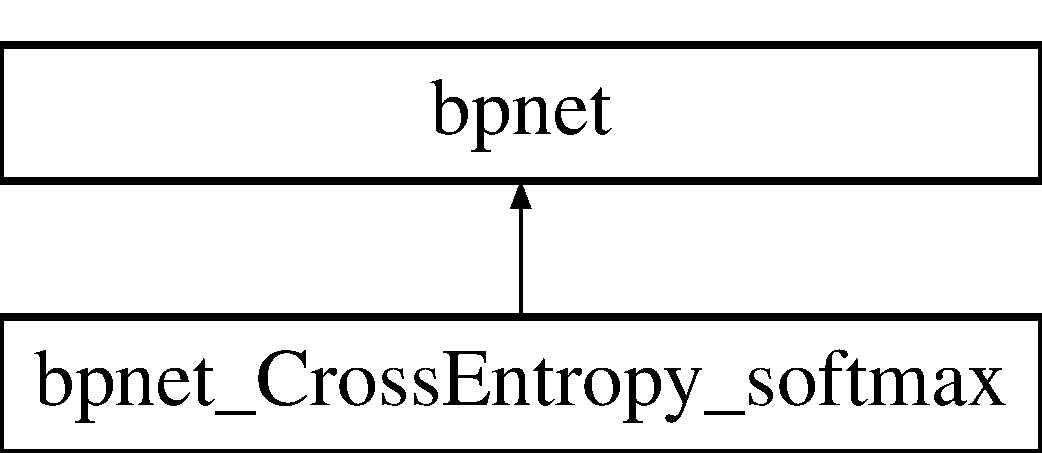
\includegraphics[height=2.000000cm]{classbpnet__CrossEntropy__softmax}
\end{center}
\end{figure}
\subsection*{Public Member Functions}
\begin{DoxyCompactItemize}
\item 
\hyperlink{classbpnet__CrossEntropy__softmax_af27dfc3aa73d018c4c5d9f27ae7057f1}{bpnet\-\_\-\-Cross\-Entropy\-\_\-softmax} (int n\-\_\-input, int n\-\_\-neurons\-\_\-in, int n\-\_\-output, std\-::vector$<$ int $>$ \-\_\-hidden\-\_\-layers, int \-\_\-n\-\_\-hidden\-\_\-layers)
\item 
\hyperlink{classbpnet__CrossEntropy__softmax_a369e61d402dde2a069fdc7cd7126c63e}{$\sim$bpnet\-\_\-\-Cross\-Entropy\-\_\-softmax} ()
\item 
void \hyperlink{classbpnet__CrossEntropy__softmax_a220ba65a1d29b86e4d200416d38c931d}{create} ()
\item 
void \hyperlink{classbpnet__CrossEntropy__softmax_a5bc91db68cdcb204fb1e46101cc731cd}{propagate} (const std\-::vector$<$ double $>$ \&input)
\item 
void \hyperlink{classbpnet__CrossEntropy__softmax_ab14df99bdcaa05a7b9c1a3b631a1662a}{update} (int layer\-\_\-index)
\item 
double \hyperlink{classbpnet__CrossEntropy__softmax_ad5945e5fb0ba6311a06833aa53023841}{train} (const std\-::vector$<$ double $>$ \&train\-\_\-data, const std\-::vector$<$ double $>$ \&train\-\_\-class, double learning\-\_\-rate, double momentum)
\item 
int \hyperlink{classbpnet__CrossEntropy__softmax_a9a4d4c77b996c83b0e881ae22868512b}{get\-\_\-n\-\_\-hidden\-\_\-layers} ()
\item 
void \hyperlink{classbpnet__CrossEntropy__softmax_aef5c2eb0db95b6bdca4cab71248f544c}{get\-\_\-output} (std\-::vector$<$ double $>$ \&input, std\-::vector$<$ double $>$ \&output)
\end{DoxyCompactItemize}
\subsection*{Additional Inherited Members}


\subsection{Detailed Description}
child class, backpropagation foward feed nerual net using croos entropy loss and softmax activation. Usually a good choice for multi-\/classification problems. 

\subsection{Constructor \& Destructor Documentation}
\hypertarget{classbpnet__CrossEntropy__softmax_af27dfc3aa73d018c4c5d9f27ae7057f1}{\index{bpnet\-\_\-\-Cross\-Entropy\-\_\-softmax@{bpnet\-\_\-\-Cross\-Entropy\-\_\-softmax}!bpnet\-\_\-\-Cross\-Entropy\-\_\-softmax@{bpnet\-\_\-\-Cross\-Entropy\-\_\-softmax}}
\index{bpnet\-\_\-\-Cross\-Entropy\-\_\-softmax@{bpnet\-\_\-\-Cross\-Entropy\-\_\-softmax}!bpnet_CrossEntropy_softmax@{bpnet\-\_\-\-Cross\-Entropy\-\_\-softmax}}
\subsubsection[{bpnet\-\_\-\-Cross\-Entropy\-\_\-softmax}]{\setlength{\rightskip}{0pt plus 5cm}bpnet\-\_\-\-Cross\-Entropy\-\_\-softmax\-::bpnet\-\_\-\-Cross\-Entropy\-\_\-softmax (
\begin{DoxyParamCaption}
\item[{int}]{n\-\_\-input, }
\item[{int}]{n\-\_\-neurons\-\_\-in, }
\item[{int}]{n\-\_\-output, }
\item[{std\-::vector$<$ int $>$}]{\-\_\-hidden\-\_\-layers, }
\item[{int}]{\-\_\-n\-\_\-hidden\-\_\-layers}
\end{DoxyParamCaption}
)\hspace{0.3cm}{\ttfamily [inline]}}}\label{classbpnet__CrossEntropy__softmax_af27dfc3aa73d018c4c5d9f27ae7057f1}
constructor initialize from base class 
\begin{DoxyParams}{Parameters}
{\em \-\_\-n\-\_\-input} & number of input variables. \\
\hline
{\em \-\_\-n\-\_\-neurons\-\_\-in} & number of neurons in input layer. \\
\hline
{\em \-\_\-n\-\_\-ouput} & number of output \\
\hline
{\em \-\_\-hidden\-\_\-layers} & hidden\-\_\-layers size vector \\
\hline
{\em \-\_\-n\-\_\-hidden\-\_\-layers} & number of hidden layers \\
\hline
\end{DoxyParams}
\hypertarget{classbpnet__CrossEntropy__softmax_a369e61d402dde2a069fdc7cd7126c63e}{\index{bpnet\-\_\-\-Cross\-Entropy\-\_\-softmax@{bpnet\-\_\-\-Cross\-Entropy\-\_\-softmax}!$\sim$bpnet\-\_\-\-Cross\-Entropy\-\_\-softmax@{$\sim$bpnet\-\_\-\-Cross\-Entropy\-\_\-softmax}}
\index{$\sim$bpnet\-\_\-\-Cross\-Entropy\-\_\-softmax@{$\sim$bpnet\-\_\-\-Cross\-Entropy\-\_\-softmax}!bpnet_CrossEntropy_softmax@{bpnet\-\_\-\-Cross\-Entropy\-\_\-softmax}}
\subsubsection[{$\sim$bpnet\-\_\-\-Cross\-Entropy\-\_\-softmax}]{\setlength{\rightskip}{0pt plus 5cm}bpnet\-\_\-\-Cross\-Entropy\-\_\-softmax\-::$\sim$bpnet\-\_\-\-Cross\-Entropy\-\_\-softmax (
\begin{DoxyParamCaption}
{}
\end{DoxyParamCaption}
)\hspace{0.3cm}{\ttfamily [inline]}}}\label{classbpnet__CrossEntropy__softmax_a369e61d402dde2a069fdc7cd7126c63e}
default destructor 

\subsection{Member Function Documentation}
\hypertarget{classbpnet__CrossEntropy__softmax_a220ba65a1d29b86e4d200416d38c931d}{\index{bpnet\-\_\-\-Cross\-Entropy\-\_\-softmax@{bpnet\-\_\-\-Cross\-Entropy\-\_\-softmax}!create@{create}}
\index{create@{create}!bpnet_CrossEntropy_softmax@{bpnet\-\_\-\-Cross\-Entropy\-\_\-softmax}}
\subsubsection[{create}]{\setlength{\rightskip}{0pt plus 5cm}void bpnet\-\_\-\-Cross\-Entropy\-\_\-softmax\-::create (
\begin{DoxyParamCaption}
{}
\end{DoxyParamCaption}
)\hspace{0.3cm}{\ttfamily [virtual]}}}\label{classbpnet__CrossEntropy__softmax_a220ba65a1d29b86e4d200416d38c931d}
create network 

Reimplemented from \hyperlink{classbpnet_a3731e200c3191fc77be85f1db2c2d4f9}{bpnet}.

\hypertarget{classbpnet__CrossEntropy__softmax_a9a4d4c77b996c83b0e881ae22868512b}{\index{bpnet\-\_\-\-Cross\-Entropy\-\_\-softmax@{bpnet\-\_\-\-Cross\-Entropy\-\_\-softmax}!get\-\_\-n\-\_\-hidden\-\_\-layers@{get\-\_\-n\-\_\-hidden\-\_\-layers}}
\index{get\-\_\-n\-\_\-hidden\-\_\-layers@{get\-\_\-n\-\_\-hidden\-\_\-layers}!bpnet_CrossEntropy_softmax@{bpnet\-\_\-\-Cross\-Entropy\-\_\-softmax}}
\subsubsection[{get\-\_\-n\-\_\-hidden\-\_\-layers}]{\setlength{\rightskip}{0pt plus 5cm}int bpnet\-\_\-\-Cross\-Entropy\-\_\-softmax\-::get\-\_\-n\-\_\-hidden\-\_\-layers (
\begin{DoxyParamCaption}
{}
\end{DoxyParamCaption}
)\hspace{0.3cm}{\ttfamily [inline]}, {\ttfamily [virtual]}}}\label{classbpnet__CrossEntropy__softmax_a9a4d4c77b996c83b0e881ae22868512b}
get number of hidden layers \begin{DoxyReturn}{Returns}
number of hidden layers 
\end{DoxyReturn}


Reimplemented from \hyperlink{classbpnet_aa35c06d999256c9aebeed4f38bca9d0f}{bpnet}.

\hypertarget{classbpnet__CrossEntropy__softmax_aef5c2eb0db95b6bdca4cab71248f544c}{\index{bpnet\-\_\-\-Cross\-Entropy\-\_\-softmax@{bpnet\-\_\-\-Cross\-Entropy\-\_\-softmax}!get\-\_\-output@{get\-\_\-output}}
\index{get\-\_\-output@{get\-\_\-output}!bpnet_CrossEntropy_softmax@{bpnet\-\_\-\-Cross\-Entropy\-\_\-softmax}}
\subsubsection[{get\-\_\-output}]{\setlength{\rightskip}{0pt plus 5cm}void bpnet\-\_\-\-Cross\-Entropy\-\_\-softmax\-::get\-\_\-output (
\begin{DoxyParamCaption}
\item[{std\-::vector$<$ double $>$ \&}]{input, }
\item[{std\-::vector$<$ double $>$ \&}]{output}
\end{DoxyParamCaption}
)\hspace{0.3cm}{\ttfamily [virtual]}}}\label{classbpnet__CrossEntropy__softmax_aef5c2eb0db95b6bdca4cab71248f544c}
get output class labels 
\begin{DoxyParams}{Parameters}
{\em input} & input data \\
\hline
{\em output} & output class label \\
\hline
\end{DoxyParams}


Reimplemented from \hyperlink{classbpnet_a9da604c278a2d583511071fdc754c9c6}{bpnet}.

\hypertarget{classbpnet__CrossEntropy__softmax_a5bc91db68cdcb204fb1e46101cc731cd}{\index{bpnet\-\_\-\-Cross\-Entropy\-\_\-softmax@{bpnet\-\_\-\-Cross\-Entropy\-\_\-softmax}!propagate@{propagate}}
\index{propagate@{propagate}!bpnet_CrossEntropy_softmax@{bpnet\-\_\-\-Cross\-Entropy\-\_\-softmax}}
\subsubsection[{propagate}]{\setlength{\rightskip}{0pt plus 5cm}void bpnet\-\_\-\-Cross\-Entropy\-\_\-softmax\-::propagate (
\begin{DoxyParamCaption}
\item[{const std\-::vector$<$ double $>$ \&}]{input}
\end{DoxyParamCaption}
)}}\label{classbpnet__CrossEntropy__softmax_a5bc91db68cdcb204fb1e46101cc731cd}
forward feeding of data 
\begin{DoxyParams}{Parameters}
{\em input} & the input data vector \\
\hline
\end{DoxyParams}
\hypertarget{classbpnet__CrossEntropy__softmax_ad5945e5fb0ba6311a06833aa53023841}{\index{bpnet\-\_\-\-Cross\-Entropy\-\_\-softmax@{bpnet\-\_\-\-Cross\-Entropy\-\_\-softmax}!train@{train}}
\index{train@{train}!bpnet_CrossEntropy_softmax@{bpnet\-\_\-\-Cross\-Entropy\-\_\-softmax}}
\subsubsection[{train}]{\setlength{\rightskip}{0pt plus 5cm}double bpnet\-\_\-\-Cross\-Entropy\-\_\-softmax\-::train (
\begin{DoxyParamCaption}
\item[{const std\-::vector$<$ double $>$ \&}]{train\-\_\-data, }
\item[{const std\-::vector$<$ double $>$ \&}]{train\-\_\-class, }
\item[{double}]{learning\-\_\-rate, }
\item[{double}]{momentum}
\end{DoxyParamCaption}
)\hspace{0.3cm}{\ttfamily [virtual]}}}\label{classbpnet__CrossEntropy__softmax_ad5945e5fb0ba6311a06833aa53023841}
training function 
\begin{DoxyParams}{Parameters}
{\em train\-\_\-data} & training data \\
\hline
{\em train\-\_\-class} & training data class label \\
\hline
{\em learning\-\_\-rate} & learning rate \\
\hline
{\em momentum} & momentum or damping factor \\
\hline
\end{DoxyParams}
\begin{DoxyReturn}{Returns}
loss value 
\end{DoxyReturn}


Reimplemented from \hyperlink{classbpnet_a653eae04b7dcfb4271421fd079849f89}{bpnet}.

\hypertarget{classbpnet__CrossEntropy__softmax_ab14df99bdcaa05a7b9c1a3b631a1662a}{\index{bpnet\-\_\-\-Cross\-Entropy\-\_\-softmax@{bpnet\-\_\-\-Cross\-Entropy\-\_\-softmax}!update@{update}}
\index{update@{update}!bpnet_CrossEntropy_softmax@{bpnet\-\_\-\-Cross\-Entropy\-\_\-softmax}}
\subsubsection[{update}]{\setlength{\rightskip}{0pt plus 5cm}void bpnet\-\_\-\-Cross\-Entropy\-\_\-softmax\-::update (
\begin{DoxyParamCaption}
\item[{int}]{layer\-\_\-index}
\end{DoxyParamCaption}
)}}\label{classbpnet__CrossEntropy__softmax_ab14df99bdcaa05a7b9c1a3b631a1662a}
update a layer 
\begin{DoxyParams}{Parameters}
{\em layer\-\_\-index} & the layer index \\
\hline
\end{DoxyParams}


The documentation for this class was generated from the following files\-:\begin{DoxyCompactItemize}
\item 
/home/jiguangshen/\-H\-P\-C\-\_\-\-Machine\-Learning/\-M\-Lcpp/src/neural\-\_\-network/nnet.\-h\item 
/home/jiguangshen/\-H\-P\-C\-\_\-\-Machine\-Learning/\-M\-Lcpp/src/neural\-\_\-network/nnet.\-cpp\end{DoxyCompactItemize}

\hypertarget{classbpnet__MSE__sigmoid}{\section{bpnet\-\_\-\-M\-S\-E\-\_\-sigmoid Class Reference}
\label{classbpnet__MSE__sigmoid}\index{bpnet\-\_\-\-M\-S\-E\-\_\-sigmoid@{bpnet\-\_\-\-M\-S\-E\-\_\-sigmoid}}
}


child class, backpropagation foward feed nerual net using mean squared error loss and sigmoid activation. Usually a good choice for binary classification problems.  




{\ttfamily \#include $<$nnet.\-h$>$}

Inheritance diagram for bpnet\-\_\-\-M\-S\-E\-\_\-sigmoid\-:\begin{figure}[H]
\begin{center}
\leavevmode
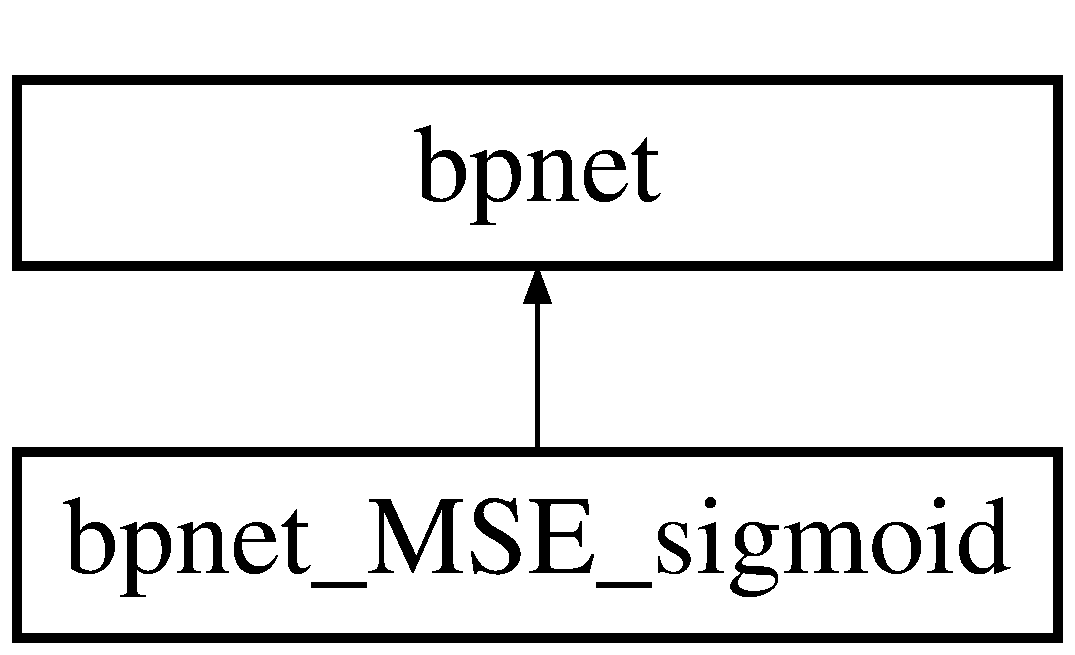
\includegraphics[height=2.000000cm]{classbpnet__MSE__sigmoid}
\end{center}
\end{figure}
\subsection*{Public Member Functions}
\begin{DoxyCompactItemize}
\item 
\hyperlink{classbpnet__MSE__sigmoid_ae9db37565d0e635570178896965a9d8c}{bpnet\-\_\-\-M\-S\-E\-\_\-sigmoid} (int n\-\_\-input, int n\-\_\-neurons\-\_\-in, int n\-\_\-output, std\-::vector$<$ int $>$ \-\_\-hidden\-\_\-layers, int \-\_\-n\-\_\-hidden\-\_\-layers)
\item 
\hyperlink{classbpnet__MSE__sigmoid_ad01362c64b5a4ad692f5a7ce77ab9f3e}{$\sim$bpnet\-\_\-\-M\-S\-E\-\_\-sigmoid} ()
\item 
void \hyperlink{classbpnet__MSE__sigmoid_a1e80df296941ce0751c8106998db05ed}{create} ()
\item 
void \hyperlink{classbpnet__MSE__sigmoid_a1ddf105554e8b9471417f624d8142077}{propagate} (const std\-::vector$<$ double $>$ \&input)
\item 
void \hyperlink{classbpnet__MSE__sigmoid_a0f934ee98b63ff4d96584cea3736a6c2}{update} (int layer\-\_\-index)
\item 
double \hyperlink{classbpnet__MSE__sigmoid_a8d69e64434b2aa992744746e5b687984}{train} (const std\-::vector$<$ double $>$ \&train\-\_\-data, const std\-::vector$<$ double $>$ \&train\-\_\-class, double learning\-\_\-rate, double momentum)
\item 
int \hyperlink{classbpnet__MSE__sigmoid_a1aab79a52a004260011a68bf50eabd28}{get\-\_\-n\-\_\-hidden\-\_\-layers} ()
\item 
void \hyperlink{classbpnet__MSE__sigmoid_ab4bf4f79ba1625fd155e7de251b57609}{get\-\_\-output} (std\-::vector$<$ double $>$ \&input, std\-::vector$<$ double $>$ \&output)
\end{DoxyCompactItemize}
\subsection*{Additional Inherited Members}


\subsection{Detailed Description}
child class, backpropagation foward feed nerual net using mean squared error loss and sigmoid activation. Usually a good choice for binary classification problems. 

\subsection{Constructor \& Destructor Documentation}
\hypertarget{classbpnet__MSE__sigmoid_ae9db37565d0e635570178896965a9d8c}{\index{bpnet\-\_\-\-M\-S\-E\-\_\-sigmoid@{bpnet\-\_\-\-M\-S\-E\-\_\-sigmoid}!bpnet\-\_\-\-M\-S\-E\-\_\-sigmoid@{bpnet\-\_\-\-M\-S\-E\-\_\-sigmoid}}
\index{bpnet\-\_\-\-M\-S\-E\-\_\-sigmoid@{bpnet\-\_\-\-M\-S\-E\-\_\-sigmoid}!bpnet_MSE_sigmoid@{bpnet\-\_\-\-M\-S\-E\-\_\-sigmoid}}
\subsubsection[{bpnet\-\_\-\-M\-S\-E\-\_\-sigmoid}]{\setlength{\rightskip}{0pt plus 5cm}bpnet\-\_\-\-M\-S\-E\-\_\-sigmoid\-::bpnet\-\_\-\-M\-S\-E\-\_\-sigmoid (
\begin{DoxyParamCaption}
\item[{int}]{n\-\_\-input, }
\item[{int}]{n\-\_\-neurons\-\_\-in, }
\item[{int}]{n\-\_\-output, }
\item[{std\-::vector$<$ int $>$}]{\-\_\-hidden\-\_\-layers, }
\item[{int}]{\-\_\-n\-\_\-hidden\-\_\-layers}
\end{DoxyParamCaption}
)\hspace{0.3cm}{\ttfamily [inline]}}}\label{classbpnet__MSE__sigmoid_ae9db37565d0e635570178896965a9d8c}
constructor initialize from base class 
\begin{DoxyParams}{Parameters}
{\em \-\_\-n\-\_\-input} & number of input variables. \\
\hline
{\em \-\_\-n\-\_\-neurons\-\_\-in} & number of neurons in input layer. \\
\hline
{\em \-\_\-n\-\_\-ouput} & number of output \\
\hline
{\em \-\_\-hidden\-\_\-layers} & hidden\-\_\-layers size vector \\
\hline
{\em \-\_\-n\-\_\-hidden\-\_\-layers} & number of hidden layers \\
\hline
\end{DoxyParams}
\hypertarget{classbpnet__MSE__sigmoid_ad01362c64b5a4ad692f5a7ce77ab9f3e}{\index{bpnet\-\_\-\-M\-S\-E\-\_\-sigmoid@{bpnet\-\_\-\-M\-S\-E\-\_\-sigmoid}!$\sim$bpnet\-\_\-\-M\-S\-E\-\_\-sigmoid@{$\sim$bpnet\-\_\-\-M\-S\-E\-\_\-sigmoid}}
\index{$\sim$bpnet\-\_\-\-M\-S\-E\-\_\-sigmoid@{$\sim$bpnet\-\_\-\-M\-S\-E\-\_\-sigmoid}!bpnet_MSE_sigmoid@{bpnet\-\_\-\-M\-S\-E\-\_\-sigmoid}}
\subsubsection[{$\sim$bpnet\-\_\-\-M\-S\-E\-\_\-sigmoid}]{\setlength{\rightskip}{0pt plus 5cm}bpnet\-\_\-\-M\-S\-E\-\_\-sigmoid\-::$\sim$bpnet\-\_\-\-M\-S\-E\-\_\-sigmoid (
\begin{DoxyParamCaption}
{}
\end{DoxyParamCaption}
)\hspace{0.3cm}{\ttfamily [inline]}}}\label{classbpnet__MSE__sigmoid_ad01362c64b5a4ad692f5a7ce77ab9f3e}
destructor 

\subsection{Member Function Documentation}
\hypertarget{classbpnet__MSE__sigmoid_a1e80df296941ce0751c8106998db05ed}{\index{bpnet\-\_\-\-M\-S\-E\-\_\-sigmoid@{bpnet\-\_\-\-M\-S\-E\-\_\-sigmoid}!create@{create}}
\index{create@{create}!bpnet_MSE_sigmoid@{bpnet\-\_\-\-M\-S\-E\-\_\-sigmoid}}
\subsubsection[{create}]{\setlength{\rightskip}{0pt plus 5cm}void bpnet\-\_\-\-M\-S\-E\-\_\-sigmoid\-::create (
\begin{DoxyParamCaption}
{}
\end{DoxyParamCaption}
)\hspace{0.3cm}{\ttfamily [virtual]}}}\label{classbpnet__MSE__sigmoid_a1e80df296941ce0751c8106998db05ed}
create network 

Reimplemented from \hyperlink{classbpnet_a3731e200c3191fc77be85f1db2c2d4f9}{bpnet}.

\hypertarget{classbpnet__MSE__sigmoid_a1aab79a52a004260011a68bf50eabd28}{\index{bpnet\-\_\-\-M\-S\-E\-\_\-sigmoid@{bpnet\-\_\-\-M\-S\-E\-\_\-sigmoid}!get\-\_\-n\-\_\-hidden\-\_\-layers@{get\-\_\-n\-\_\-hidden\-\_\-layers}}
\index{get\-\_\-n\-\_\-hidden\-\_\-layers@{get\-\_\-n\-\_\-hidden\-\_\-layers}!bpnet_MSE_sigmoid@{bpnet\-\_\-\-M\-S\-E\-\_\-sigmoid}}
\subsubsection[{get\-\_\-n\-\_\-hidden\-\_\-layers}]{\setlength{\rightskip}{0pt plus 5cm}int bpnet\-\_\-\-M\-S\-E\-\_\-sigmoid\-::get\-\_\-n\-\_\-hidden\-\_\-layers (
\begin{DoxyParamCaption}
{}
\end{DoxyParamCaption}
)\hspace{0.3cm}{\ttfamily [inline]}, {\ttfamily [virtual]}}}\label{classbpnet__MSE__sigmoid_a1aab79a52a004260011a68bf50eabd28}
get number of hidden layers \begin{DoxyReturn}{Returns}
number of hidden layers 
\end{DoxyReturn}


Reimplemented from \hyperlink{classbpnet_aa35c06d999256c9aebeed4f38bca9d0f}{bpnet}.

\hypertarget{classbpnet__MSE__sigmoid_ab4bf4f79ba1625fd155e7de251b57609}{\index{bpnet\-\_\-\-M\-S\-E\-\_\-sigmoid@{bpnet\-\_\-\-M\-S\-E\-\_\-sigmoid}!get\-\_\-output@{get\-\_\-output}}
\index{get\-\_\-output@{get\-\_\-output}!bpnet_MSE_sigmoid@{bpnet\-\_\-\-M\-S\-E\-\_\-sigmoid}}
\subsubsection[{get\-\_\-output}]{\setlength{\rightskip}{0pt plus 5cm}void bpnet\-\_\-\-M\-S\-E\-\_\-sigmoid\-::get\-\_\-output (
\begin{DoxyParamCaption}
\item[{std\-::vector$<$ double $>$ \&}]{input, }
\item[{std\-::vector$<$ double $>$ \&}]{output}
\end{DoxyParamCaption}
)\hspace{0.3cm}{\ttfamily [virtual]}}}\label{classbpnet__MSE__sigmoid_ab4bf4f79ba1625fd155e7de251b57609}
get output class labels 
\begin{DoxyParams}{Parameters}
{\em input} & input data \\
\hline
{\em output} & output class label \\
\hline
\end{DoxyParams}


Reimplemented from \hyperlink{classbpnet_a9da604c278a2d583511071fdc754c9c6}{bpnet}.

\hypertarget{classbpnet__MSE__sigmoid_a1ddf105554e8b9471417f624d8142077}{\index{bpnet\-\_\-\-M\-S\-E\-\_\-sigmoid@{bpnet\-\_\-\-M\-S\-E\-\_\-sigmoid}!propagate@{propagate}}
\index{propagate@{propagate}!bpnet_MSE_sigmoid@{bpnet\-\_\-\-M\-S\-E\-\_\-sigmoid}}
\subsubsection[{propagate}]{\setlength{\rightskip}{0pt plus 5cm}void bpnet\-\_\-\-M\-S\-E\-\_\-sigmoid\-::propagate (
\begin{DoxyParamCaption}
\item[{const std\-::vector$<$ double $>$ \&}]{input}
\end{DoxyParamCaption}
)}}\label{classbpnet__MSE__sigmoid_a1ddf105554e8b9471417f624d8142077}
forward feeding of data 
\begin{DoxyParams}{Parameters}
{\em input} & the input data vector \\
\hline
\end{DoxyParams}
\hypertarget{classbpnet__MSE__sigmoid_a8d69e64434b2aa992744746e5b687984}{\index{bpnet\-\_\-\-M\-S\-E\-\_\-sigmoid@{bpnet\-\_\-\-M\-S\-E\-\_\-sigmoid}!train@{train}}
\index{train@{train}!bpnet_MSE_sigmoid@{bpnet\-\_\-\-M\-S\-E\-\_\-sigmoid}}
\subsubsection[{train}]{\setlength{\rightskip}{0pt plus 5cm}double bpnet\-\_\-\-M\-S\-E\-\_\-sigmoid\-::train (
\begin{DoxyParamCaption}
\item[{const std\-::vector$<$ double $>$ \&}]{train\-\_\-data, }
\item[{const std\-::vector$<$ double $>$ \&}]{train\-\_\-class, }
\item[{double}]{learning\-\_\-rate, }
\item[{double}]{momentum}
\end{DoxyParamCaption}
)\hspace{0.3cm}{\ttfamily [virtual]}}}\label{classbpnet__MSE__sigmoid_a8d69e64434b2aa992744746e5b687984}
training function 
\begin{DoxyParams}{Parameters}
{\em train\-\_\-data} & training data \\
\hline
{\em train\-\_\-class} & training data class label \\
\hline
{\em learning\-\_\-rate} & learning rate \\
\hline
{\em momentum} & momentum or damping factor \\
\hline
\end{DoxyParams}
\begin{DoxyReturn}{Returns}
loss value 
\end{DoxyReturn}


Reimplemented from \hyperlink{classbpnet_a653eae04b7dcfb4271421fd079849f89}{bpnet}.

\hypertarget{classbpnet__MSE__sigmoid_a0f934ee98b63ff4d96584cea3736a6c2}{\index{bpnet\-\_\-\-M\-S\-E\-\_\-sigmoid@{bpnet\-\_\-\-M\-S\-E\-\_\-sigmoid}!update@{update}}
\index{update@{update}!bpnet_MSE_sigmoid@{bpnet\-\_\-\-M\-S\-E\-\_\-sigmoid}}
\subsubsection[{update}]{\setlength{\rightskip}{0pt plus 5cm}void bpnet\-\_\-\-M\-S\-E\-\_\-sigmoid\-::update (
\begin{DoxyParamCaption}
\item[{int}]{layer\-\_\-index}
\end{DoxyParamCaption}
)}}\label{classbpnet__MSE__sigmoid_a0f934ee98b63ff4d96584cea3736a6c2}
update a layer 
\begin{DoxyParams}{Parameters}
{\em layer\-\_\-index} & the layer index \\
\hline
\end{DoxyParams}


The documentation for this class was generated from the following files\-:\begin{DoxyCompactItemize}
\item 
/home/jiguangshen/\-H\-P\-C\-\_\-\-Machine\-Learning/\-M\-Lcpp/src/neural\-\_\-network/nnet.\-h\item 
/home/jiguangshen/\-H\-P\-C\-\_\-\-Machine\-Learning/\-M\-Lcpp/src/neural\-\_\-network/nnet.\-cpp\end{DoxyCompactItemize}

\hypertarget{structdataframe}{\section{dataframe Struct Reference}
\label{structdataframe}\index{dataframe@{dataframe}}
}


The data framework for classification problems. It defines the way to load data and handle categorical class variables and display data info.  




{\ttfamily \#include $<$dataframe.\-h$>$}

Inheritance diagram for dataframe\-:\begin{figure}[H]
\begin{center}
\leavevmode
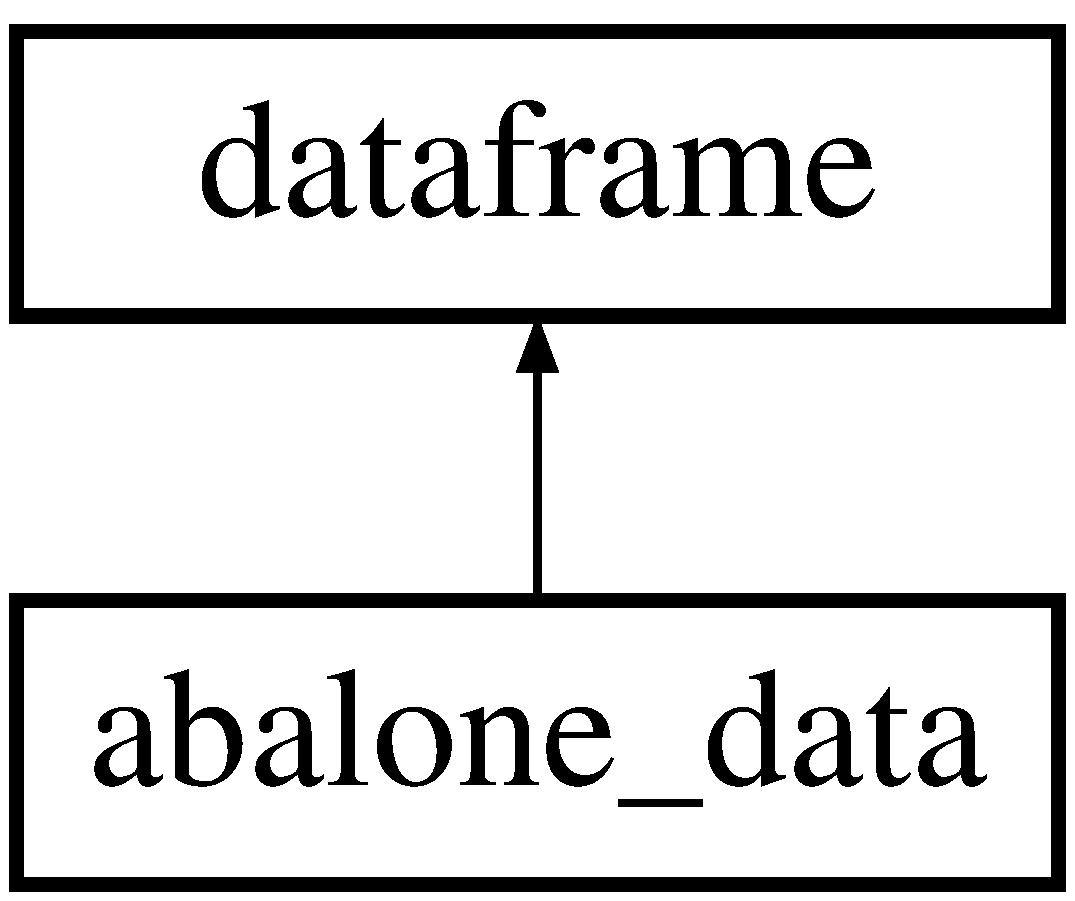
\includegraphics[height=2.000000cm]{structdataframe}
\end{center}
\end{figure}
\subsection*{Public Member Functions}
\begin{DoxyCompactItemize}
\item 
\hyperlink{structdataframe_a4ddfcbd8b4c6a38a5439811e9a8621e8}{dataframe} ()
\item 
virtual \hyperlink{structdataframe_a3e5a7cfc9408d92321f6ba8ea7635178}{$\sim$dataframe} ()
\item 
virtual void \hyperlink{structdataframe_ae108c949f6f3f89c7ed000e90c3a2e64}{load} (std\-::string \&path)
\item 
virtual void \hyperlink{structdataframe_ac71cab6be91e8cb90d8efa88e6866b83}{data\-\_\-info} ()
\end{DoxyCompactItemize}
\subsection*{Public Attributes}
\begin{DoxyCompactItemize}
\item 
\hypertarget{structdataframe_ad3f184a47c59346533a0194b6c06e52c}{int {\bfseries n\-\_\-instance}}\label{structdataframe_ad3f184a47c59346533a0194b6c06e52c}

\item 
\hypertarget{structdataframe_a5a79b2e10c24de75717c87c2f74f6809}{int {\bfseries n\-\_\-attributes}}\label{structdataframe_a5a79b2e10c24de75717c87c2f74f6809}

\item 
std\-::vector$<$ std\-::vector\\*
$<$ double $>$ $>$ \hyperlink{structdataframe_af6f4f8d2ada43ba75b9b2a726d8dbf91}{all\-\_\-label}
\item 
std\-::vector$<$ std\-::vector\\*
$<$ double $>$ $>$ \hyperlink{structdataframe_a8d76966d6bccec17ca513628319c8527}{all\-\_\-feature}
\end{DoxyCompactItemize}


\subsection{Detailed Description}
The data framework for classification problems. It defines the way to load data and handle categorical class variables and display data info. 

\subsection{Constructor \& Destructor Documentation}
\hypertarget{structdataframe_a4ddfcbd8b4c6a38a5439811e9a8621e8}{\index{dataframe@{dataframe}!dataframe@{dataframe}}
\index{dataframe@{dataframe}!dataframe@{dataframe}}
\subsubsection[{dataframe}]{\setlength{\rightskip}{0pt plus 5cm}dataframe\-::dataframe (
\begin{DoxyParamCaption}
{}
\end{DoxyParamCaption}
)\hspace{0.3cm}{\ttfamily [inline]}}}\label{structdataframe_a4ddfcbd8b4c6a38a5439811e9a8621e8}
constructor \hypertarget{structdataframe_a3e5a7cfc9408d92321f6ba8ea7635178}{\index{dataframe@{dataframe}!$\sim$dataframe@{$\sim$dataframe}}
\index{$\sim$dataframe@{$\sim$dataframe}!dataframe@{dataframe}}
\subsubsection[{$\sim$dataframe}]{\setlength{\rightskip}{0pt plus 5cm}virtual dataframe\-::$\sim$dataframe (
\begin{DoxyParamCaption}
{}
\end{DoxyParamCaption}
)\hspace{0.3cm}{\ttfamily [inline]}, {\ttfamily [virtual]}}}\label{structdataframe_a3e5a7cfc9408d92321f6ba8ea7635178}
destructor 

\subsection{Member Function Documentation}
\hypertarget{structdataframe_ac71cab6be91e8cb90d8efa88e6866b83}{\index{dataframe@{dataframe}!data\-\_\-info@{data\-\_\-info}}
\index{data\-\_\-info@{data\-\_\-info}!dataframe@{dataframe}}
\subsubsection[{data\-\_\-info}]{\setlength{\rightskip}{0pt plus 5cm}virtual void dataframe\-::data\-\_\-info (
\begin{DoxyParamCaption}
{}
\end{DoxyParamCaption}
)\hspace{0.3cm}{\ttfamily [inline]}, {\ttfamily [virtual]}}}\label{structdataframe_ac71cab6be91e8cb90d8efa88e6866b83}
print data info 

Reimplemented in \hyperlink{structiris__data_a6e149a32e92f33cbeb1a1ccdb5bf75f1}{iris\-\_\-data}, and \hyperlink{structbanknote__data_afbe0c062a0fc69f8edd74dbe17571f4a}{banknote\-\_\-data}.

\hypertarget{structdataframe_ae108c949f6f3f89c7ed000e90c3a2e64}{\index{dataframe@{dataframe}!load@{load}}
\index{load@{load}!dataframe@{dataframe}}
\subsubsection[{load}]{\setlength{\rightskip}{0pt plus 5cm}virtual void dataframe\-::load (
\begin{DoxyParamCaption}
\item[{std\-::string \&}]{path}
\end{DoxyParamCaption}
)\hspace{0.3cm}{\ttfamily [inline]}, {\ttfamily [virtual]}}}\label{structdataframe_ae108c949f6f3f89c7ed000e90c3a2e64}
load data from file 
\begin{DoxyParams}{Parameters}
{\em path} & string path to file \\
\hline
\end{DoxyParams}


Reimplemented in \hyperlink{structiris__data_a23c106db87bef4ab1ef81d99d78f07c7}{iris\-\_\-data}, and \hyperlink{structbanknote__data_a2915563eeee2f721994ce9c5daaf4c93}{banknote\-\_\-data}.



\subsection{Member Data Documentation}
\hypertarget{structdataframe_a8d76966d6bccec17ca513628319c8527}{\index{dataframe@{dataframe}!all\-\_\-feature@{all\-\_\-feature}}
\index{all\-\_\-feature@{all\-\_\-feature}!dataframe@{dataframe}}
\subsubsection[{all\-\_\-feature}]{\setlength{\rightskip}{0pt plus 5cm}std\-::vector$<$std\-::vector$<$double$>$ $>$ dataframe\-::all\-\_\-feature}}\label{structdataframe_a8d76966d6bccec17ca513628319c8527}
feature sets \hypertarget{structdataframe_af6f4f8d2ada43ba75b9b2a726d8dbf91}{\index{dataframe@{dataframe}!all\-\_\-label@{all\-\_\-label}}
\index{all\-\_\-label@{all\-\_\-label}!dataframe@{dataframe}}
\subsubsection[{all\-\_\-label}]{\setlength{\rightskip}{0pt plus 5cm}std\-::vector$<$std\-::vector$<$double$>$ $>$ dataframe\-::all\-\_\-label}}\label{structdataframe_af6f4f8d2ada43ba75b9b2a726d8dbf91}
all class label which is transformed into numerical values 

The documentation for this struct was generated from the following file\-:\begin{DoxyCompactItemize}
\item 
/home/jiguangshen/\-H\-P\-C\-\_\-\-Machine\-Learning/\-M\-Lcpp/src/examples/dataframe.\-h\end{DoxyCompactItemize}

\hypertarget{structlayer}{\section{layer Struct Reference}
\label{structlayer}\index{layer@{layer}}
}


the layer structure which consists of neurons and an activation function.  




{\ttfamily \#include $<$layer.\-h$>$}

Inheritance diagram for layer\-:\begin{figure}[H]
\begin{center}
\leavevmode
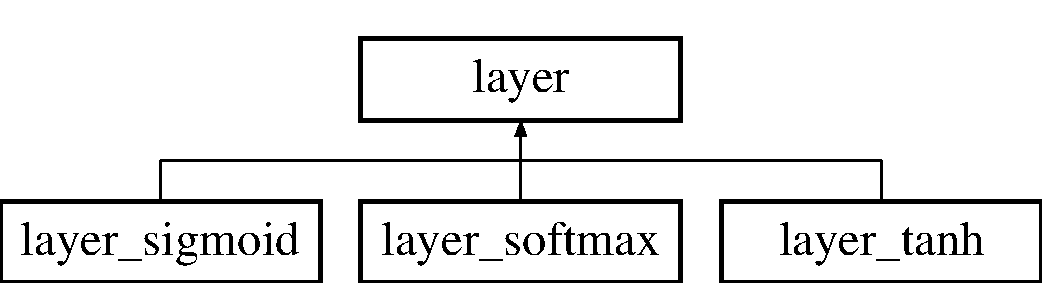
\includegraphics[height=2.000000cm]{structlayer}
\end{center}
\end{figure}
\subsection*{Public Member Functions}
\begin{DoxyCompactItemize}
\item 
\hyperlink{structlayer_a95796de3b5f8aa07f49effa03a03f6f8}{layer} ()
\item 
virtual \hyperlink{structlayer_ae0781f14cd91478477526183951eb052}{$\sim$layer} ()
\item 
void \hyperlink{structlayer_a50ca540d57f99add95b7e92c96498810}{create} (int \-\_\-n\-\_\-input, int \-\_\-n\-\_\-neuron)
\item 
virtual void \hyperlink{structlayer_aacf7297d77c1ea2933d5551636f7c9ad}{calculate} ()=0
\end{DoxyCompactItemize}
\subsection*{Public Attributes}
\begin{DoxyCompactItemize}
\item 
\hypertarget{structlayer_a370f3ea69cfa52d599d8bb107276122d}{std\-::vector$<$ \hyperlink{structneuron}{neuron} $>$ {\bfseries neurons}}\label{structlayer_a370f3ea69cfa52d599d8bb107276122d}

\item 
\hypertarget{structlayer_aefd4997e805a4f4c3db2b5415104d215}{std\-::vector$<$ double $>$ {\bfseries layerinput}}\label{structlayer_aefd4997e805a4f4c3db2b5415104d215}

\item 
\hypertarget{structlayer_a17b545f98fb35b4b856e3e0c8d9a0876}{int {\bfseries n\-\_\-neuron}}\label{structlayer_a17b545f98fb35b4b856e3e0c8d9a0876}

\item 
\hypertarget{structlayer_a8323a6ef4cab8f81515ca964b79034fe}{int {\bfseries n\-\_\-input}}\label{structlayer_a8323a6ef4cab8f81515ca964b79034fe}

\end{DoxyCompactItemize}


\subsection{Detailed Description}
the layer structure which consists of neurons and an activation function. 

\subsection{Constructor \& Destructor Documentation}
\hypertarget{structlayer_a95796de3b5f8aa07f49effa03a03f6f8}{\index{layer@{layer}!layer@{layer}}
\index{layer@{layer}!layer@{layer}}
\subsubsection[{layer}]{\setlength{\rightskip}{0pt plus 5cm}layer\-::layer (
\begin{DoxyParamCaption}
{}
\end{DoxyParamCaption}
)}}\label{structlayer_a95796de3b5f8aa07f49effa03a03f6f8}
constructor \hypertarget{structlayer_ae0781f14cd91478477526183951eb052}{\index{layer@{layer}!$\sim$layer@{$\sim$layer}}
\index{$\sim$layer@{$\sim$layer}!layer@{layer}}
\subsubsection[{$\sim$layer}]{\setlength{\rightskip}{0pt plus 5cm}virtual layer\-::$\sim$layer (
\begin{DoxyParamCaption}
{}
\end{DoxyParamCaption}
)\hspace{0.3cm}{\ttfamily [inline]}, {\ttfamily [virtual]}}}\label{structlayer_ae0781f14cd91478477526183951eb052}
destructor 

\subsection{Member Function Documentation}
\hypertarget{structlayer_aacf7297d77c1ea2933d5551636f7c9ad}{\index{layer@{layer}!calculate@{calculate}}
\index{calculate@{calculate}!layer@{layer}}
\subsubsection[{calculate}]{\setlength{\rightskip}{0pt plus 5cm}virtual void layer\-::calculate (
\begin{DoxyParamCaption}
{}
\end{DoxyParamCaption}
)\hspace{0.3cm}{\ttfamily [pure virtual]}}}\label{structlayer_aacf7297d77c1ea2933d5551636f7c9ad}
pure virtual function to calculate layer output based on the activation function 

Implemented in \hyperlink{structlayer__softmax_addf2fcfd6b5c0131e2429f49835bf8e8}{layer\-\_\-softmax}, \hyperlink{structlayer__tanh_aa06a41d4ddfa798cafd99cf1e22f1a48}{layer\-\_\-tanh}, and \hyperlink{structlayer__sigmoid_a04a54d415eb5412fcd78478b3e113f3f}{layer\-\_\-sigmoid}.

\hypertarget{structlayer_a50ca540d57f99add95b7e92c96498810}{\index{layer@{layer}!create@{create}}
\index{create@{create}!layer@{layer}}
\subsubsection[{create}]{\setlength{\rightskip}{0pt plus 5cm}void layer\-::create (
\begin{DoxyParamCaption}
\item[{int}]{\-\_\-n\-\_\-input, }
\item[{int}]{\-\_\-n\-\_\-neuron}
\end{DoxyParamCaption}
)}}\label{structlayer_a50ca540d57f99add95b7e92c96498810}
create a layer 
\begin{DoxyParams}{Parameters}
{\em \-\_\-n\-\_\-input} & the number of inputs \\
\hline
{\em \-\_\-n\-\_\-neuron} & the number of neurons in the layer \\
\hline
\end{DoxyParams}


The documentation for this struct was generated from the following files\-:\begin{DoxyCompactItemize}
\item 
/home/jiguangshen/\-H\-P\-C\-\_\-\-Machine\-Learning/\-M\-Lcpp/src/neural\-\_\-network/layer.\-h\item 
/home/jiguangshen/\-H\-P\-C\-\_\-\-Machine\-Learning/\-M\-Lcpp/src/neural\-\_\-network/layer.\-cpp\end{DoxyCompactItemize}

\hypertarget{structlayer__sigmoid}{\section{layer\-\_\-sigmoid Struct Reference}
\label{structlayer__sigmoid}\index{layer\-\_\-sigmoid@{layer\-\_\-sigmoid}}
}


The layer with a sigmoid activation.  




{\ttfamily \#include $<$layer.\-h$>$}

Inheritance diagram for layer\-\_\-sigmoid\-:\begin{figure}[H]
\begin{center}
\leavevmode
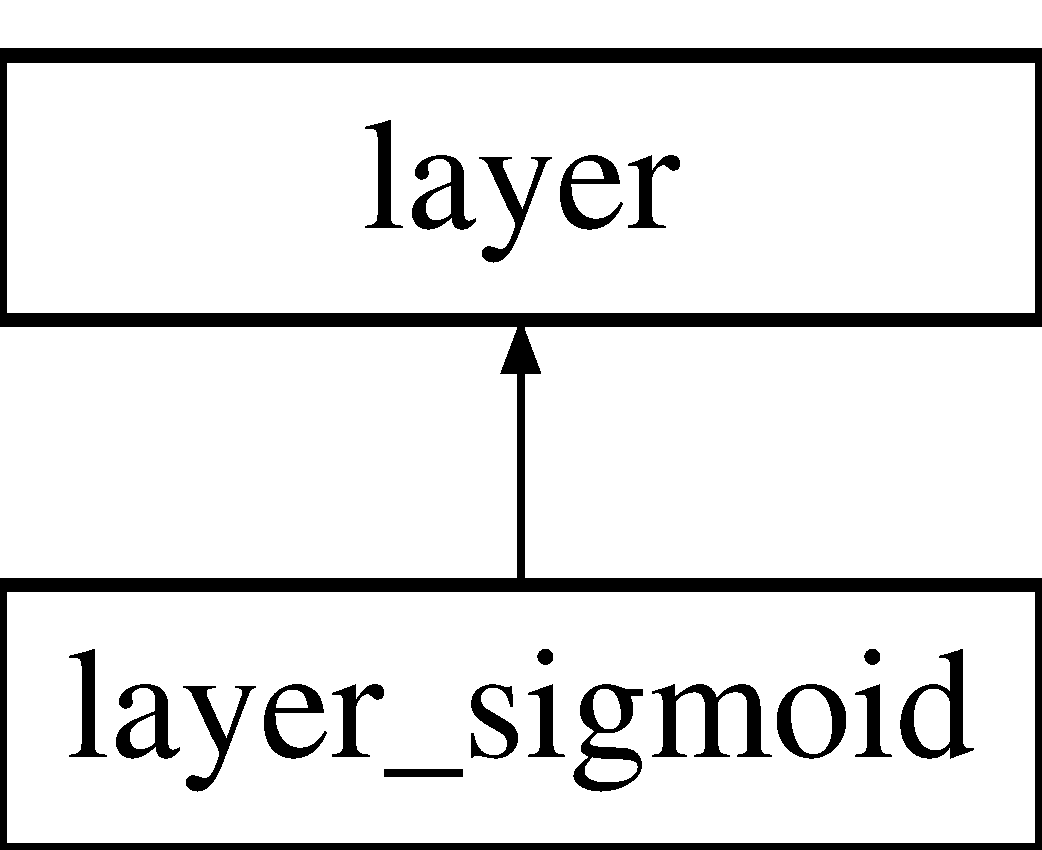
\includegraphics[height=2.000000cm]{structlayer__sigmoid}
\end{center}
\end{figure}
\subsection*{Public Member Functions}
\begin{DoxyCompactItemize}
\item 
void \hyperlink{structlayer__sigmoid_a04a54d415eb5412fcd78478b3e113f3f}{calculate} ()
\end{DoxyCompactItemize}
\subsection*{Additional Inherited Members}


\subsection{Detailed Description}
The layer with a sigmoid activation. 

\subsection{Member Function Documentation}
\hypertarget{structlayer__sigmoid_a04a54d415eb5412fcd78478b3e113f3f}{\index{layer\-\_\-sigmoid@{layer\-\_\-sigmoid}!calculate@{calculate}}
\index{calculate@{calculate}!layer_sigmoid@{layer\-\_\-sigmoid}}
\subsubsection[{calculate}]{\setlength{\rightskip}{0pt plus 5cm}void layer\-\_\-sigmoid\-::calculate (
\begin{DoxyParamCaption}
{}
\end{DoxyParamCaption}
)\hspace{0.3cm}{\ttfamily [virtual]}}}\label{structlayer__sigmoid_a04a54d415eb5412fcd78478b3e113f3f}
pure virtual function to calculate layer output based on the activation function 

Implements \hyperlink{structlayer_aacf7297d77c1ea2933d5551636f7c9ad}{layer}.



The documentation for this struct was generated from the following files\-:\begin{DoxyCompactItemize}
\item 
/home/jiguangshen/\-H\-P\-C\-\_\-\-Machine\-Learning/\-M\-Lcpp/src/neural\-\_\-network/layer.\-h\item 
/home/jiguangshen/\-H\-P\-C\-\_\-\-Machine\-Learning/\-M\-Lcpp/src/neural\-\_\-network/layer.\-cpp\end{DoxyCompactItemize}

\hypertarget{structlayer__softmax}{\section{layer\-\_\-softmax Struct Reference}
\label{structlayer__softmax}\index{layer\-\_\-softmax@{layer\-\_\-softmax}}
}
Inheritance diagram for layer\-\_\-softmax\-:\begin{figure}[H]
\begin{center}
\leavevmode
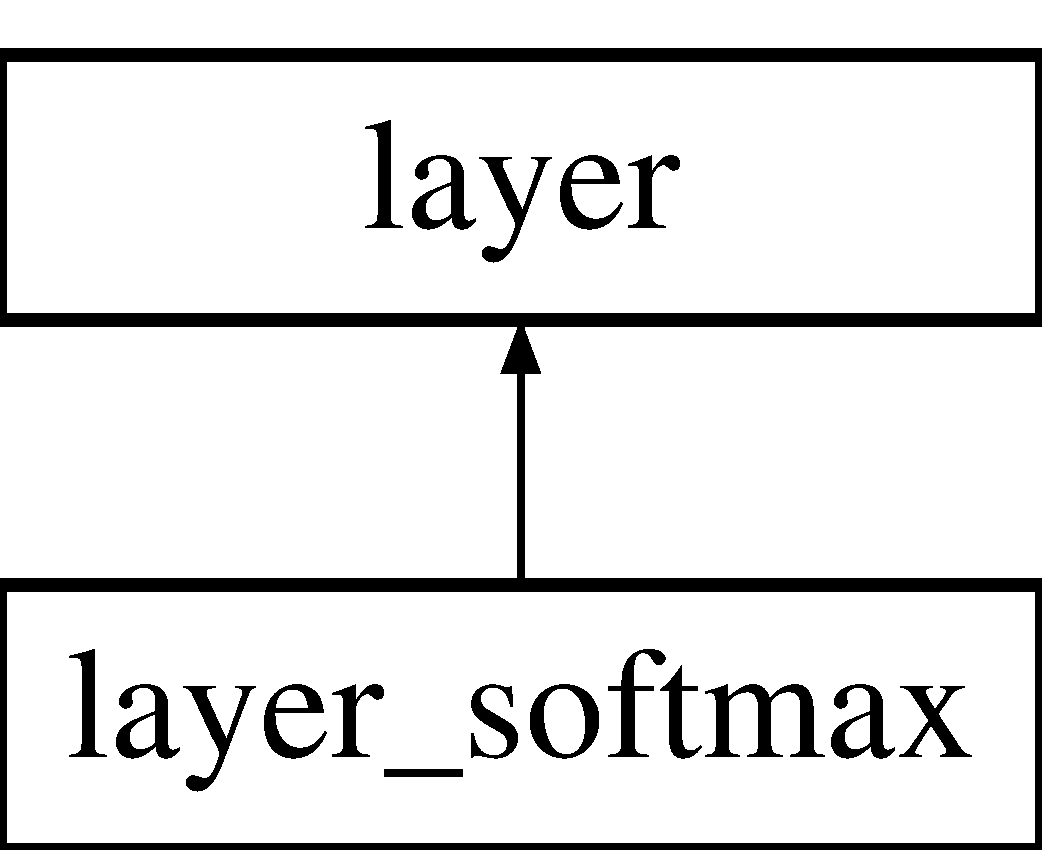
\includegraphics[height=2.000000cm]{structlayer__softmax}
\end{center}
\end{figure}
\subsection*{Public Member Functions}
\begin{DoxyCompactItemize}
\item 
\hypertarget{structlayer__softmax_addf2fcfd6b5c0131e2429f49835bf8e8}{void {\bfseries calculate} ()}\label{structlayer__softmax_addf2fcfd6b5c0131e2429f49835bf8e8}

\end{DoxyCompactItemize}
\subsection*{Additional Inherited Members}


The documentation for this struct was generated from the following files\-:\begin{DoxyCompactItemize}
\item 
/home/jiguangshen/\-H\-P\-C\-\_\-\-Machine\-Learning/\-M\-Lcpp/src/neural\-\_\-network/layer.\-h\item 
/home/jiguangshen/\-H\-P\-C\-\_\-\-Machine\-Learning/\-M\-Lcpp/src/neural\-\_\-network/layer.\-cpp\end{DoxyCompactItemize}

\hypertarget{structlayer__tanh}{\section{layer\-\_\-tanh Struct Reference}
\label{structlayer__tanh}\index{layer\-\_\-tanh@{layer\-\_\-tanh}}
}


The layer with a tanh activation.  




{\ttfamily \#include $<$layer.\-h$>$}

Inheritance diagram for layer\-\_\-tanh\-:\begin{figure}[H]
\begin{center}
\leavevmode
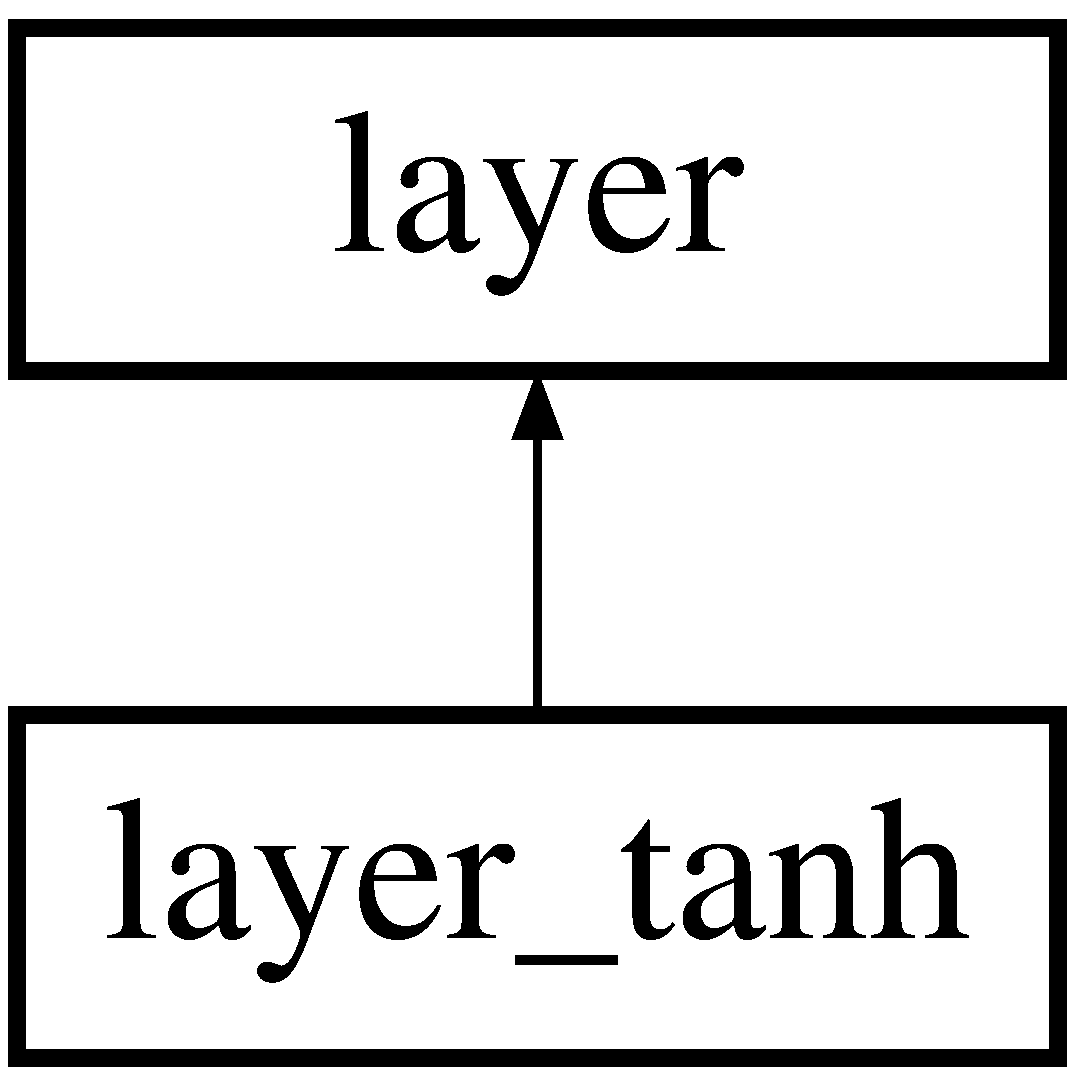
\includegraphics[height=2.000000cm]{structlayer__tanh}
\end{center}
\end{figure}
\subsection*{Public Member Functions}
\begin{DoxyCompactItemize}
\item 
void \hyperlink{structlayer__tanh_aa06a41d4ddfa798cafd99cf1e22f1a48}{calculate} ()
\end{DoxyCompactItemize}
\subsection*{Additional Inherited Members}


\subsection{Detailed Description}
The layer with a tanh activation. 

\subsection{Member Function Documentation}
\hypertarget{structlayer__tanh_aa06a41d4ddfa798cafd99cf1e22f1a48}{\index{layer\-\_\-tanh@{layer\-\_\-tanh}!calculate@{calculate}}
\index{calculate@{calculate}!layer_tanh@{layer\-\_\-tanh}}
\subsubsection[{calculate}]{\setlength{\rightskip}{0pt plus 5cm}void layer\-\_\-tanh\-::calculate (
\begin{DoxyParamCaption}
{}
\end{DoxyParamCaption}
)\hspace{0.3cm}{\ttfamily [virtual]}}}\label{structlayer__tanh_aa06a41d4ddfa798cafd99cf1e22f1a48}
pure virtual function to calculate layer output based on the activation function 

Implements \hyperlink{structlayer_aacf7297d77c1ea2933d5551636f7c9ad}{layer}.



The documentation for this struct was generated from the following files\-:\begin{DoxyCompactItemize}
\item 
/home/jiguangshen/\-H\-P\-C\-\_\-\-Machine\-Learning/\-M\-Lcpp/src/neural\-\_\-network/layer.\-h\item 
/home/jiguangshen/\-H\-P\-C\-\_\-\-Machine\-Learning/\-M\-Lcpp/src/neural\-\_\-network/layer.\-cpp\end{DoxyCompactItemize}

\hypertarget{structneuron}{\section{neuron Struct Reference}
\label{structneuron}\index{neuron@{neuron}}
}
\subsection*{Public Member Functions}
\begin{DoxyCompactItemize}
\item 
\hypertarget{structneuron_abbe656fe98d44f42741b9b3412c05187}{void {\bfseries create} (int n\-\_\-input)}\label{structneuron_abbe656fe98d44f42741b9b3412c05187}

\item 
\hypertarget{structneuron_a6751788971a339ccc522333f740ffd41}{void {\bfseries activate} ()}\label{structneuron_a6751788971a339ccc522333f740ffd41}

\item 
\hypertarget{structneuron_adbea299710f3a6402e83433b3c0cabf9}{void {\bfseries deactivate} ()}\label{structneuron_adbea299710f3a6402e83433b3c0cabf9}

\end{DoxyCompactItemize}
\subsection*{Public Attributes}
\begin{DoxyCompactItemize}
\item 
\hypertarget{structneuron_a46dd6f29c430390f623f708e12fdf333}{std\-::vector$<$ double $>$ {\bfseries weights}}\label{structneuron_a46dd6f29c430390f623f708e12fdf333}

\item 
\hypertarget{structneuron_adbb698db478b03d1df7da41d977a8690}{std\-::vector$<$ double $>$ {\bfseries deltas}}\label{structneuron_adbb698db478b03d1df7da41d977a8690}

\item 
\hypertarget{structneuron_ae47a1f9995c0649c2d5811692c1d294f}{double {\bfseries output}}\label{structneuron_ae47a1f9995c0649c2d5811692c1d294f}

\item 
\hypertarget{structneuron_a9ab850dc68643bc01d84c6bbef9640a9}{double {\bfseries bias}}\label{structneuron_a9ab850dc68643bc01d84c6bbef9640a9}

\item 
\hypertarget{structneuron_a02ae7cb21e0edaf78e96b687ae10c2b6}{double {\bfseries w\-\_\-bias}}\label{structneuron_a02ae7cb21e0edaf78e96b687ae10c2b6}

\item 
\hypertarget{structneuron_a23ae47a4501a58d5f9ac6b5d37622e9a}{bool {\bfseries active}}\label{structneuron_a23ae47a4501a58d5f9ac6b5d37622e9a}

\end{DoxyCompactItemize}


The documentation for this struct was generated from the following files\-:\begin{DoxyCompactItemize}
\item 
/home/jiguangshen/\-H\-P\-C\-\_\-\-Machine\-Learning/\-M\-Lcpp/src/neural\-\_\-network/neuron.\-h\item 
/home/jiguangshen/\-H\-P\-C\-\_\-\-Machine\-Learning/\-M\-Lcpp/src/neural\-\_\-network/neuron.\-cpp\end{DoxyCompactItemize}

%--- End generated contents ---

% Index
\newpage
\phantomsection
\addcontentsline{toc}{chapter}{Index}
\printindex

\end{document}
